\chapter{Vorarbeit}
\label{c:vorarbeit}


\section{Recherche zu Browser-Extensions}
\label{s:recherchebrowserextensions}

\subsection{Extension-Programmierung allgemein}
\label{ss:extensionprogallg}

Unter einer Extension versteht man ein Programm, welches den Browser um neue Funktionen ergänzt. Durch eigene Oberflächen oder Manipulation der Website erleichtern diese Erweiterungen das Nutzen des Browser.

Im Gegensatz zu Plug-Ins haben Extensions Zugriff auf Browser-spezielle Funktionen und sind in der Lage über die Webseite hinaus zu agieren. Plug-Ins werden direkt in eine Webseite eingebettet und sind auf diese beschränkt. Der Oberbegriff „Add-on“ wird heutzutage Hauptsächlich als Synonym für Extension verwendet.

Jeder größere Browser stellt eine Plattform zur Verfügung auf denen Extensions angeboten und installiert werden können. In der Regel sind Diese kostenlos. Wird eine Applikation nicht auf der Plattform angeboten oder dient sie zu Entwicklungszwecken, kann diese auch manuell aus externen Quelle installiert werden.

Extensions werden in HTML, JavaScript und CSS implementiert. Dabei können alle Bibliotheken verwendet werden, welche den Browserstandards für Extensions entsprechen. Kapitel 2.3.2 befasst sich genauer damit, welche Bedingungen für diese Bibliotheken in Google Chrome gelten.

Bekannte Beispiele sind Werbeblocker wie UBlock Origin und VPN-Anwendungen wie Hola.

\subsection{Existieren bereits vergleichbare Extensions}
\label{ss:vergleichbareextensions}

Gesucht wurde nach einer Extension die auf der Play Store Seite den Nutzer datenschutzrelevante Informationen zu den angebotenen Apps liefert, Eine Datenschutzwertung im Playstore vergibt oder den Nutzer Apps nach Berechtigungen die Apps vorschlägt.
Extensions werden nach ihrer Kurzbeschreibung in den Suchergebnissen überprüft und bei nicht eindeutig Aufgabenbeschreibung die Infoseite aufgerufen(Bsp. Safe.ad im Web Store „ecosystem“).Nur deutsche und englische  Ergebnisse werden berücksichtigt.

Die Recherche hat ergeben, dass unter den genannten Suchkriterien keine Chrome oder Firefox Extension gefunden wurde die Aufgabenbereich der geplanten Extension abdeckt. Einige aufgeführte Beispiele implementieren einen Teil der geplanten Funktion (Umsortierung, Tracker checken) , aber keine Extension erfüllt alle gewünschten Aufgaben.


\subsection{Vergleich führender Browser als Plattform für die Extension}
\label{ss:vergleichbrowser}
Die getroffene Auswahl des Browsers als Plattform für die Entwicklung der Extension basiert hauptsächlich auf den aktuellen Marktanteilen. Google Chrome führt mit ca. 71\%, gefolgt von Mozilla Firefox mit 9,5\%, Microsoft Internet Explorer mit ca. 5,7\%, Apple Safari mit ca. 5\%, Microsoft Edge mit 4,4\% und Opera mit ca. 2,4\%.

\begin{figure}[ht]
	\centering
	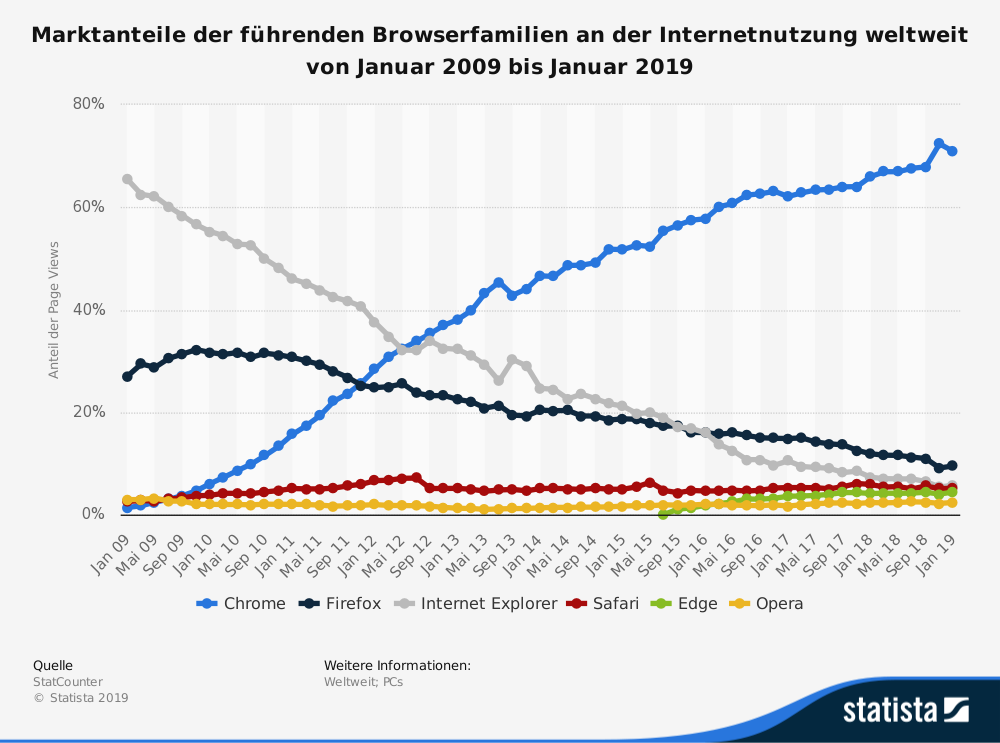
\includegraphics[width=1\textwidth]{pics/MarktanteileBrowser.png}
	\caption{StatCounter. n.d. Marktanteile der führenden Browserfamilien an der Internetnutzung weltweit von Januar 2009 bis Januar 2019. Statista. Zugriff am 4. März 2019. Verfügbar unter \url{https://de.statista.com/statistik/daten/studie/157944/umfrage/marktanteile-der-browser-bei-der-internetnutzung-weltweit-seit-2009/}.}
	\label{marktanteilebrowser}
\end{figure}
Aufgrund mangelnder Relevanz der Extension für Safari-Nutzer, sowie der Obsoleszenz des Internet Explorers, wurden diese Browser nicht weiter berücksichtigt.

Google Chrome ist den verbleibenden Alternativen Mozilla Firefox, Microsoft Edge und Opera im Punkt Marktanteile weit voraus und somit die gewählte Plattform zur Entwicklung der Extension.

Unabhängig der Implementierung bieten sowohl Mozilla\footnote{\url{https://developer.mozilla.org/en-US/docs/Mozilla/Add-ons/WebExtensions/Porting_a_Google_Chrome_extension}}, als auch Edge\footnote{\url{https://docs.microsoft.com/en-us/microsoft-edge/extensions/guides/porting-chrome-extensions}} eine intuitive Lösung zur Portierung der fertigen Google Chrome-Extension.

\section{PrivacyGuard}
\label{s:pguard}

\subsection{Vorstellung}
\label{ss:vorstellung}
Das Forschungsprojekt Privacy Guard\footnote{\url{https://datenschutz-scanner.de/das-projekt.html}} wurde im Januar 2016 durch das Bundesministerium für Bildung und Forschung ins Leben gerufen. Das Institut für Angewandte Informatik\footnote{\url{https://infai.org/}}, die mediaTest digital GmbH\footnote{\url{https://appvisory.com/company}}, die Quadriga Hochschule Berlin\footnote{\url{https://www.quadriga-hochschule.com/}} und die selbstregulierung informationswirtschaft e.V.\footnote{\url{https://sriw.de/}} haben gemeinsam Möglichkeiten entwickelt, Verbraucher auf die Verarbeitung ihrer Daten durch Handy-Applikationen aufmerksam zu machen. Dabei werden Vor- und Nachteile einzelner Aspekte der Datenverarbeitung erläutert und, bei Bedarf, Gegenmaßnahmen empfohlen.

\glqq Ziel [...] ist die Erleichterung des Selbstdatenschutzes für Verbraucher auf mobilen Endgeräten.\grqq{}(https://datenschutz-scanner.de/das-projekt.html,Stand 4.3.2019)

Die Ergebnisse des Projekts teilen sich in 3 Kategorien ein. Im Rahmen der Datenbeschaffung entstanden verschiedene Werkzeuge um Informationen über Apps zu extrahieren. Besonderer Wert wurde hier auf verlinkte Datenschutzerklärungen im Playstore und in der später installierten App auf dem Handy gelegt. Desweiteren wurden die Datenschutzerklärungen mittels eines entwickelten Pre-Tagging Tools, aber auch manuell annotiert, um die Verarbeitung der Texte zu optimieren.

Zur Datenverarbeitung entstand ein Backend\footnote{\url{https://pgadmin.datenschutz-scanner.de/api/docs.html}}, welches auf Anfrage der Bundle-ID einer App alle analysierten Daten übergibt. Dieses Backend bildet die Grundlage für die Datenvisualisierung von PGuard und ist die Schnittstelle der Informationen für die Browser-Extension.

Mit dem Projektabschluss im Juni 2018 stellte PrivacyGuard eine Webseite zur Analyse von Datenschutzerklärungen und Apps zur Verfügung\footnote{\url{https://dseanalyser.pguard-tools.de/}}. Als Prototypen entstanden zusätzlich eine App zur Analyse aller auf dem Handy installierten Applikationen auf ihren Datenschutz und die in dieser Arbeit behandelte Browser-Extension zur Visualisierung der, durch das Projekt gewonnenen, Informationen über Apps im PlayStore.

\subsection{API-Anbindung für die Extension}
\label{ss:apianbindung}

Sämtliche, von der Extension visualisierte, Daten werden über die Schnittstelle des Backends angefragt. Dazu benötigt die API mindestens eine Bundle-ID der App, Priorität und die Ausführtlichkeit der Antwort.

Je höher die Anfrage priorisiert ist, um so eher wird sie vom Backend verarbeitet. 
Bei einer hohen Ausführlichkeit umfassen die angeforderten Informationen komplette Datenschutzerklärungen und alle Metainformationen zur Datenbeschaffung. Dagegen beinhaltet eine Antwort mit niedriger Ausführlichkeit lediglich Sprache, Quelle und Extraktionsdatum der Datenschutzerklärung, sowie die Nummer der geltenden Infofelder mit jeweiligen Textpassagen aus der Datenschutzerklärung.

Für den Anwendungsfall der Browser-Extension besteht eine hohe Priorität um Wartezeiten möglichst gering zu halten. Dagegen reicht eine niedrige Ausführlichkeit zur Darstellung der nötigen Informationen für den Verbraucher. Zusätzlich bleibt so der Datenverkehr der Extension eher gering.

Die Infofelder sind der Hauptinformationsträger der Schnittstelle. Sie sind in 31 Eigenschaften unterteilt und können eine sogenannten "rote Linie" sein. Das bedeutet, dass bei Besitz dieser Eigenschaft, die entsprechende App potentiell gegen ein Gesetz verstößt. Folgenden Infofelder sind im Rahmen des PrivacyGuard Forschungsprojekts zur Beurteilung von Apps entstanden(siehe Abbildung \ref{tabelleInfofelder} und Abbildung \ref{tabelleInfofelderzwei}).

\begin{table}[h]
	\begin{tabular}{p{0.5cm}L{9.0cm}R{2.1cm}}
		\toprule
		\textbf{Nr.}		&	\textbf{Bezeichnung}		&	\textbf{rote Linie}	\\
		\midrule
		1	&	Ihre Zahlungsdaten werden unverschlüsselt übermittelt	&	Ja		\\
		2	&	Die App hat Internetzugriff	&	Nein	\\
		3	&	Die App benennt keine Kontaktmöglichkeit für datenschutzrechtliche Anliegen	&	Ja	\\
		4	&	Ihre Login-Daten werden unverschlüsselt übermittelt	&	Ja	\\
		5	&	Die App stellt keine Datenschutzerklärung auf Deutsch bereit	&	Nein	\\
		6	&	Die Datenschutzerklärung verwendet ungenaue Formulierungen	&	Nein	\\
		7	&	Die Verschlüsselung der App ist unsicher	&	Nein	\\
		8	&	Die App nutzt Standortdaten	&	Nein	\\
		9	&	Die Datenschutzerklärung kann geändert werden, ohne Sie hierüber zu informieren	&	Ja	\\
		10	&	Das über Sie erstellte Profil wird durch öffentliche Informationen über Sie ergänzt	&	Nein	\\
		11	&	Ihre Daten werden durch Dienstleister verarbeitet	&	Nein	\\
		12	&	Die App integriert Werbenetzwerke	&	Nein	\\
		13	&	Die App erhebt eine Vielzahl an Geräteinformationen	&	Nein	\\
		14	&	Die App stellt die Datenschutzerklärung erst nach Start der App bereit	&	Nein	\\
		15	&	Die App hat Zugriff auf Ihr Adressbuch	&	Nein	\\
		\bottomrule
	\end{tabular}
	\caption{Übersicht der Infofelder von PrivacyGuard}
	\label{tabelleInfofelder}
\end{table}

\begin{table}[h]
	\begin{tabular}{p{0.5cm}L{9.0cm}R{2.1cm}}
		\toprule
		\textbf{Nr.}		&	\textbf{Bezeichnung}		&	\textbf{rote Linie}	\\
		\midrule
		16	&	Die App enthält Malware	&	Ja	\\
		17	&	Die App übermittelt Daten an Dritte	&	Nein	\\
		18	&	Die App erhebt statische Gerätekennungen	&	Nein	\\
		19	&	Die App verarbeitet Daten, die für die Funktion der App nicht erforderlich sind	&	Nein	\\
		20	&	Die App verarbeitet Daten, die ausdrücklich ausgeschlossen wurden	&	Ja	\\
		21	&	Die App ermöglicht einer Vielzahl von Drittanbietern Zugriff auf Ihre Nutzungsdaten	&	Nein	\\
		22	&	Es wird ein Profil über Sie erstellt	&	Nein	\\
		23	&	Ihre Daten werden in der Unternehmensgruppe geteilt	&	Nein	\\
		24	&	Die App kann sich im Hintergrund unbemerkt aktualisieren	&	Nein	\\
		25	&	Die Herkunft der App ist unbekannt	&	Nein	\\
		26	&	Die App stellt keine Datenschutzerklärung bereit	&	Ja	\\
		27	&	Ihre Daten werden für personalisierte Werbung genutzt	&	Nein	\\
		28	&	Die App klärt nicht ordnungsgemäß über Datenverarbeitungen im Ausland auf	&	Nein	\\
		29	&	Die App stellt unterschiedliche Datenschutzerklärungen in der App und im App-Store bereit	&	Ja	\\
		30	&	Ihre Daten werden über die App veröffentlicht	&	Nein	\\
		31	&	Die Sprachsteuerung ist dauerhaft im Hintergrund aktiv	&	Nein	\\
		\bottomrule
	\end{tabular}
	\caption{Übersicht der Infofelder von PrivacyGuard}
	\label{tabelleInfofelderzwei}
\end{table}

\section{Implementierung einer Google Chrome Extension}
\label{s:implementierung}

\subsection{Eigenschaften}
\label{ss:eigenschaften}

Die Architektur einer Google Chrome Extension stellt ein Paket aus mehreren Dateien dar und ist vergleichbar mit anderen Web-Technologien wie zum Beispiel Webseiten.

Grundvoraussetzung für eine funktionierende Extension ist die manifest.json, welche nötigen Informationen für den Browser bereitstellt und festlegt mit welchen Dateien und Rechten die Extension aufgebaut ist. Hinzu kommt mindestens eine HTML-Datei zur Darstellung der Inhalte und mindestens ein Skript zur Umsetzung der Funktionalität. Erweitert werden diese oft durch CSS-Dateien.

Externe Bibliotheken wie JQuery können ebenfalls eingebunden werden, müssen aber aufgrund der Policies\footnote{\url{https://developer.chrome.com/webstore/program_policies}} von Google Chrome vollumfänglich lokal vorliegen. Mehr dazu Im nächsten Abschnitt.

Die Manifest-Datei ist im JSON-Format aufgebaut und beinhaltet sämtliche Informationen über die Extension. Wichtige Punkte sind Name der Extension, Beschreibung, Rechte und Aufbau. Unter Rechten oder „permissions“ werden alle APIs aufgelistet, welche die Extension benötigt um ordnungsgemäß zu funktionieren. Bevor ein Nutzer später die Extension installiert, muss er diesen „permissions“ zustimmen.

Der Aufbau wird im Punkt „content scripts“ in drei Eigenschaften unterteilt: unter welchem URL sind die Skripte aktiv, welche Skripte sind dort aktiv und welche CSS-Dateien werden dort von der Extension eingesetzt.

HTML-Dateien werden als „User-Interface Elemente“ zusammengefasst und beinhalten im Normalfall eine popup.html zur Darstellung des Fensters der Extension in der oberen rechten Ecke des Browser-Fensters (BILD?). Je nach Funktionsumfang können weitere UI-Elemente eingebunden sein, um zum Beispiel die besuchte Webseite zu erweitern.

Die vorhandenen Skripte werden normalerweise in zwei Kategorien eingeteilt. Das sogenannte „Background-Skript“ dient als Event-Handler und kommuniziert zwischen Extension und Browser. Alle restlichen Skripte sind „Content-Skripte“. Sie beinhalten die eigentliche Funktionalität der Extension. 

\subsection{Funktionsumfang und Richtlinien}
\label{ss:funktionsumfang}

Google setzt verschiedene Qualitätsansprüche an die Entwicklung einer Extension. Den Leitfaden bildet dabei das sogenannten \glqq single purpose\grqq{}-Prinzip\footnote{\url{https://developer.chrome.com/extensions/single_purpose}}. Das heißt, jede Anwendung muss auf sich entweder auf ein bestimmtes Thema fokussieren, wie zum Beispiel Datenschutzerklärungen und darf zu diesem Thema verschiedene Funktionen anbieten. Oder die Extension konzentriert sich auf eine bestimmte Funktion des Browser, wie zum Beispiel die Startseite und darf dort Inhalte zu mehreren Themen implementieren.

Ein weiterer Aspekt, der mit dem \glqq single purpose\grqq{}-Prinzip zusammenhängt, ist die Reichweite der Extension. Google unterscheidet hier zwischen \glqq page-action\grqq{} und \glqq browser-action\grqq{}.

\glqq page-action\grqq{} bedeutet, dass das Icon der Extension lediglich auf einer bestimmten Seite aktiv ist und soll den Nutzer darauf hinweisen, wo sich die Erweiterung einschaltet. Icons mit \glqq browser-action\grqq{} sind permanent aktiv und zeigen somit, dass die Extension seitenübergreifende Funktionen hat.

Auch inhaltlich gibt es bestimmte Richtlinien\footnote{\url{https://developer.chrome.com/webstore/program_policies}} zu beachten. Die \glqq Content Policies \grqq{} untersagen die Einbindung von Material mit sexuell expliziten Inhalten, Gewaltdarstellungen, \glqq Hate Speech \grqq{}, Identitätsbetrug, Urheberrechtsverletzung, Schadsoftware, Glücksspiel, Spam oder anderen illegalen Aktivitäten.

Ist Werbung ein Bestandteil der Erweiterung, unterliegen diese Inhalte ebenfalls strengen Auflagen. Der Nutzer muss in der Lage sein, die Werbung ohne Probleme zu entfernen, zum Beispiel durch Deinstallation der Extension. Werbeanzeigen dürfen keine Programmfunktionen versperren, imitieren oder andere schädliche Absichten verfolgen. Sind Anzeigen von externen Webseiten geschalten, muss das klar ausgewiesen sein.

Erhebt, speichert oder verarbeitet die Extension sensitive Nutzerdaten, muss der Entwickler das entsprechend deklarieren und trägt Verantwortung für die Sicherheit der Daten. In diesem Zusammenhang benötigt die Anwendung eine eigene Datenschutzerklärung.
\subsection{Darstellung im Browser}
\label{ss:darstellung}

Die Extension wird an mehreren Stellen im Browser integriert. Dabei besitzt jedes installierte Programm ein Icon in der Adresszeile des Browsers (Abbildung \ref{browser1}). Dieses Element dient als Steuerelement für Funktionen der Erweiterung, wie zum Beispiel das Aktivieren und Deaktivieren der Extension. Ein ausgegrautes Icon bedeutet dabei, dass die Extension inaktiv ist, bzw. das die zugehörige Webseite nicht in diesem Tab geöffnet ist.
\begin{figure}[ht]
	\centering
	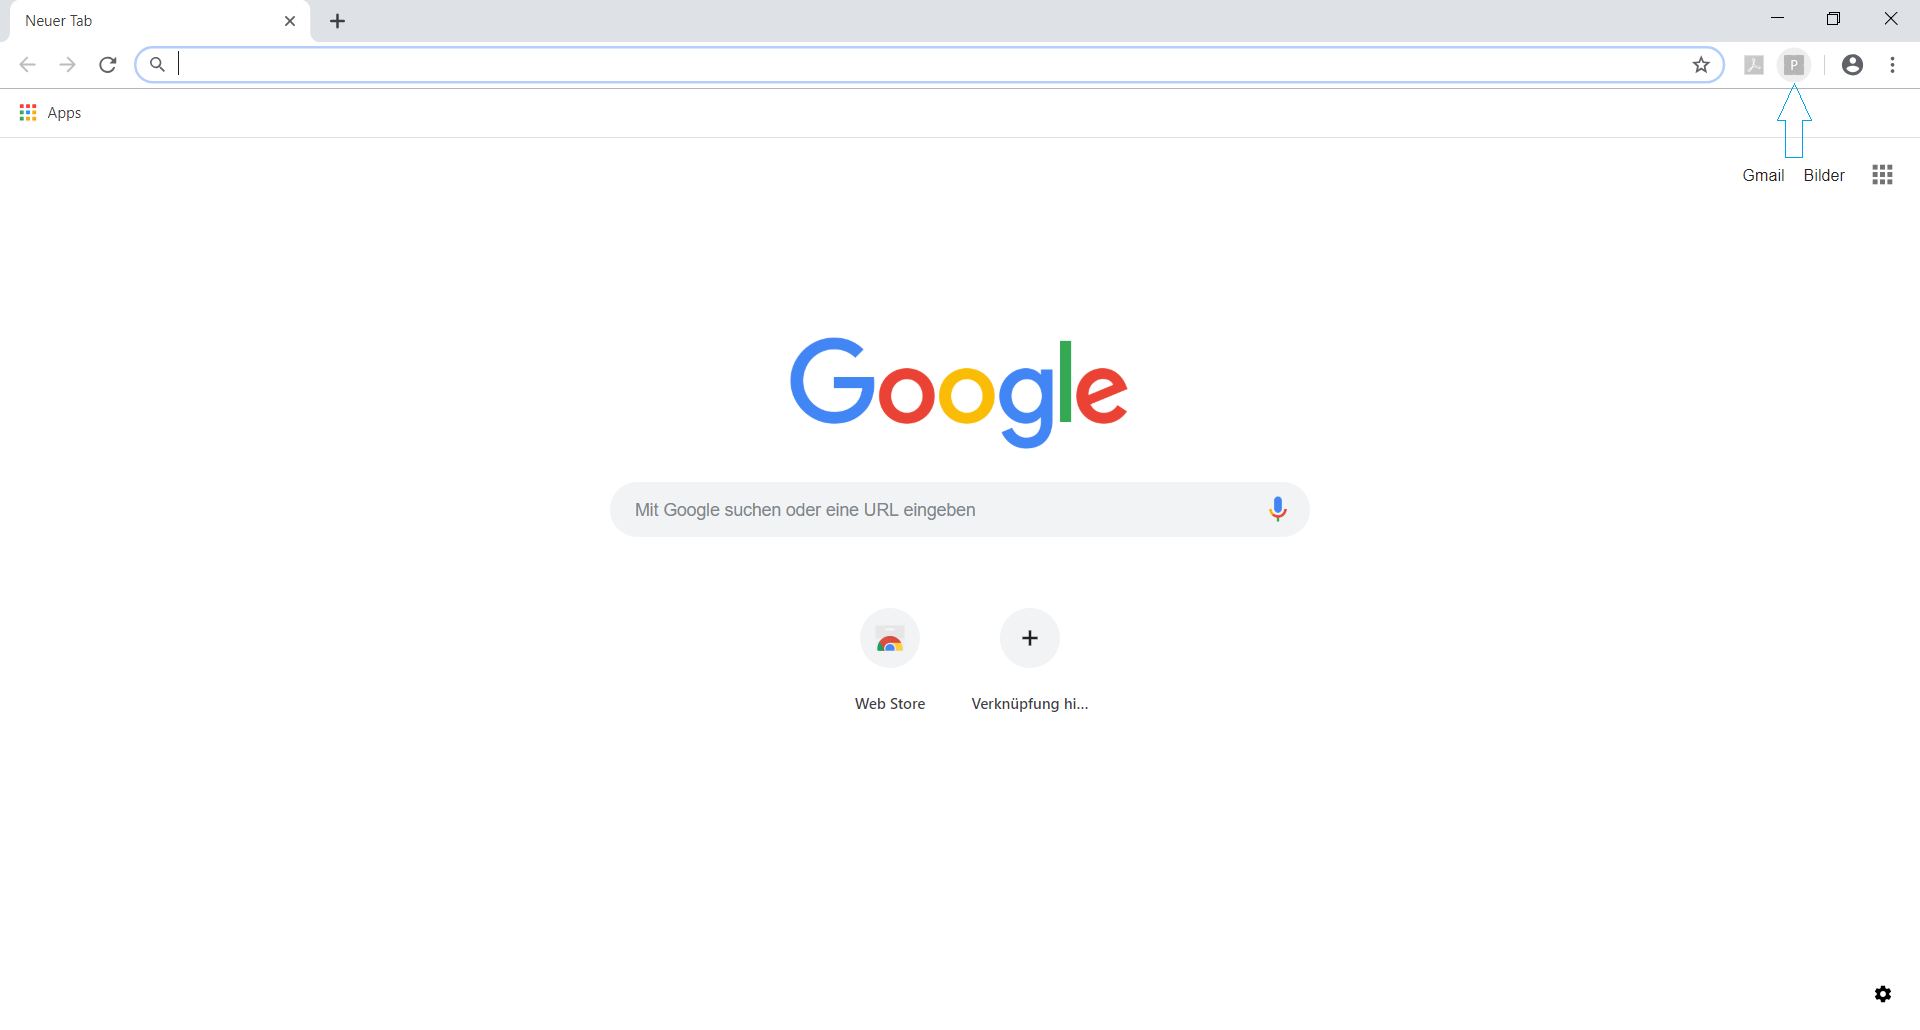
\includegraphics[width=1\textwidth]{pics/browser1.png}
	\caption{Browser-Extension Icon in der Adresszeile}
	\label{browser1}
\end{figure}

Eine weitere Möglichkeit Inhalte und Funktionen der Erweiterung zu verwalten, ohne dafür Template des Icons zu verwenden, ist die dedizierte Optionenseite\footnote{\url{https://developer.chrome.com/extensions/options}}. Diese kommt vor allem bei umfangreicheren Browser-Extensions vor.

Alle restlichen Elemente werden direkt in die angezeigte Webseite integriert und erweitern die Anzeige beliebig nach Funktion der Extension.(REF)
\section{Caching-Methoden}
\label{s:cachingmethoden}

\subsection{Anforderungen}
\label{ss:cacheanforderungen}

Diese Arbeit beschäftigt sich damit, welche Caching-Methoden für Browser-Extensions geeignet sind. Der Fokus liegt hierbei auf den in Aufgabe \ref{s:aufgabenstellung} beschriebenen Anwendungsfall. Darauß ergeben sich folgende Anforderungen an den Speicher:

Performanz spielt eine große Rolle, da dem Nutzer alle gespeicherten Daten der Extension zeitgleich zum Abschluss der Ladezeit der Webseite zur Verfügung stehen sollen. Werden Daten mit Verzögerung auf der Webseite dargestellt oder Verlängert der Prozess sogar die initiale Ladezeit, hat das eine beträchtliche Auswirkung auf die Nutzererfahrung. So zeigt eine Studie von Google Research auf dem Jahr 2017\footnote{\url{https://www.thinkwithgoogle.com/marketing-resources/data-measurement/mobile-page-speed-new-industry-benchmarks/}}, dass die Absprungrate sich bei Ladezeiten von über zwei Sekunden stark erhöht.

Aufgrund der Schnelllebigkeit der Informationen, müssen diese nicht über einen längeren Zeitraum abgespeichert werden. Außerdem verarbeitet die Browser-Extension keine Daten weiter. Verlorene Einträge können so durch eine erneute Anfrage verlustfrei ersetzt werden. 

Lastverteilung ist eine der Hauptanforderungen an die Caching-Methoden in dieser Arbeit. Da alle Daten über ein zentrales Backend abgerufen werden, besteht die Gefahr des Flaschenhalseffekts. Zudem sollen allgemein möglichst wenig Anfragen an externe Quellen gestellt werden, um so das Risiko zu vermeiden, auf Antworten von Server zu warten.

Alle Daten, die im Cache abgelegt werden sind durch PrivacyGuard gewonnene Informationen über die einzelnen Applikationen und beziehen sich nicht auf den Nutzer der Extension. Es werden also keine sensiblen Daten im Cache abgelegt. Somit besteht kein Bedarf an Sicherheitsmaßnahmen wie etwa die Verschlüsselung der Daten.

Die Datenvisualisierung der Extension ist überschaubar und auch die zu Grunde liegende Datenstruktur der API ist einfach aufgebaut. Dadurch kann auf komplexe Datenbankstrukturen oder zusätzliche Frameworks verzichtet werden.

\subsection{Caching-Methoden und deren Eigenschaften}
\label{ss:methodeneigenschaften}

Um zu evaluieren, welche Caching-Methode am besten für den beschriebenen Anwendungsfall geeignet ist, befasst sich dieses Kapitel mit der Auflistung aller möglichen Speicherfunktionen für Browser-Extensions. Die dazu aufgelisteten Eigenschaften dienen als Vergleich für die spätere Vorauswahl der Methoden.
Als Quelle für Teile der Recherche diente das Buch von Raymond Camden \glqq Client-Side Data Storgae \grqq{}

Alle Daten der Extension sollen im Browser gespeichert werden. Datenbanken auf externen Servern bieten keinen Mehrwert, da die Informationen vom Backend nicht noch verarbeitet, personalisiert, oder gesichert werden müssen. In diesem Fall dient das Backend als Datenbank, die durch lokale Speicherprozesse entlastet werden soll.

Cookies sind kleine Textspeicher die normalerweise von Webseiten in Browsern genutzt werden, um Informationen über den Besucher zu speichern. Sie besitzen meist eine kurze Lebensdauer und werden über HTTP-Header übertragen. Auch Browser-Extensions können Cookies nutzen\footnote{\url{https://developer.chrome.com/extensions/cookies}}, um Informationen zu speichern. Das Buch verweist darauf, dass man bis zu 50 Cookies mit einer Gesamtgröße von 4KB pro Domäne ohne bedenken nutzen kann.
Jedoch genießen Cookies, unter anderem aufgrund der EU-Richtlinie\footnote{\url{https://eur-lex.europa.eu/LexUriServ/LexUriServ.do?uri=CELEX:32002L0058:de:HTML}}, keinen guten Ruf. Webseiten müssen sich in der Regel vor Gebrauch die Genehmigung des Nutzers einholen. Dies könnte also auch bei Extension zu rechtlichen Problemen führen. Außerdem blockieren viele Nutzer diese Cookies eben aus datenschutzrechtlichen Gründen.

Die Web Storage API\footnote{\url{https://developer.mozilla.org/en-US/docs/Web/API/Web_Storage_API}} ist eine einheitlich Methode von mehreren Browser, Daten lokal zu speichern. Pro Domäne verfügt der Web Storage über 5-10MB, je nach Browser. Dabei besteht jede Einheit aus einem key-value-Paar, welches Daten in Form von Strings speichern kann. Die Web Storage API ist unterteilt in \glqq local storage\grqq{} und \glqq session storage\grqq{}. Während beim session storage alle Daten nur solange gespeichert sind, bis der Browser wieder geschlossen wird, bleiben die Daten beim local storage solange bestehen, bis sie manuell überschrieben oder gelöscht werden.

Mit der IndexedDB API\footnote{\url{https://developer.mozilla.org/de/docs/IndexedDB}} ist die Extension in der Lage eine domainspezifische Datenbank zu erstellen. Diese Datenbank besteht aus sogenannten \glqq Object Stores\grqq{}, welche Tabellen mit flexiblen Datentypen beinhalten können. Die Speicherkapazität wird nicht exakt definiert und ist abhängig von der Größe der Festplatte\footnote{\url{https://developer.mozilla.org/de/docs/IndexedDB/Browser_storage_limits_and_eviction_criteria}}. So liegt der verfügbare Speicher zwischen 10MB und 50\% des freien Festplattenspeichers. IndexedDB wird nicht noch komplett unterstützt und gilt als vergleichsweise komplexe API.

Ergänzend zu erwähnen ist die SQLite basierte Datenbank Web SQL. Seit 2010 wird diese Spezifikation von dem World-Wide-Web-Konsortium allerdings nicht mehr zur Implementierung empfohlen und gilt seit jeher als veraltet.
















